\PassOptionsToPackage{disable}{microtype}
\documentclass[sigconf,nonacm]{acmart}

\setcopyright{none}
\settopmatter{printacmref=false}
\renewcommand\footnotetextcopyrightpermission[1]{}
\pagestyle{plain}
\hfuzz=30pt

\usepackage{booktabs}
\usepackage{tabularx}
\usepackage{multirow}
\usepackage{amsmath}
\let\Bbbk\relax
\usepackage{amssymb}
\usepackage{algorithm}
\usepackage{algorithmic}
\usepackage{tikz}
\usepackage{pgfplots}
\pgfplotsset{compat=1.18}
\usepackage{url}
\urlstyle{rm}

\usetikzlibrary{arrows.meta,positioning,calc,shapes.geometric,
                decorations.pathreplacing,patterns,fit,backgrounds}

\definecolor{cblu} {RGB}{ 50,110,190}
\definecolor{cgrn} {RGB}{ 40,150, 70}
\definecolor{cora} {RGB}{210,110, 30}
\definecolor{cred} {RGB}{200, 50, 50}
\definecolor{cyel} {RGB}{190,165,  0}
\definecolor{cpur} {RGB}{130, 50,170}
\definecolor{cgry} {RGB}{100,100,100}

\begin{CCSXML}
<ccs2012>
  <concept>
    <concept_id>10002978.10003006.10003008</concept_id>
    <concept_desc>Security and privacy~Intrusion/anomaly detection and malware mitigation</concept_desc>
    <concept_significance>500</concept_significance>
  </concept>
  <concept>
    <concept_id>10010583.10010600.10010628</concept_id>
    <concept_desc>Computer systems organization~Cyber-physical systems</concept_desc>
    <concept_significance>500</concept_significance>
  </concept>
  <concept>
    <concept_id>10010147.10010178.10010219.10010220</concept_id>
    <concept_desc>Computing methodologies~Causal reasoning and diagnostics</concept_desc>
    <concept_significance>300</concept_significance>
  </concept>
  <concept>
    <concept_id>10010147.10010257.10010293</concept_id>
    <concept_desc>Computing methodologies~Neural networks</concept_desc>
    <concept_significance>300</concept_significance>
  </concept>
</ccs2012>
\end{CCSXML}

\ccsdesc[500]{Security and privacy~Intrusion/anomaly detection and malware mitigation}
\ccsdesc[500]{Computer systems organization~Cyber-physical systems}
\ccsdesc[300]{Computing methodologies~Causal reasoning and diagnostics}
\ccsdesc[300]{Computing methodologies~Neural networks}

\title{TwinAlign: Cross-Domain Consistency Detection of Reality-Drift and Adversarial Synchronisation Attacks in Digital Twin Cyber-Physical Systems}

\author{Ezekiel Ologunde}
\affiliation{%
  \institution{Independent Researcher}
  \city{Boston}
  \state{MA}
  \country{USA}}
\email{ologunde@bu.edu}

\begin{abstract}
\sloppy
Digital twins synchronise real-world cyber-physical systems with
virtual representations for monitoring, prediction, and increasingly
direct control. The deployment trajectory has accelerated sharply in
2024--2026: smart-city digital twins (Singapore Virtual Singapore,
Helsinki 3D City Information Model), industrial-process digital twins
(Siemens Xcelerator, GE Predix, Bosch Connected Industry),
healthcare digital twins (FDA-cleared cardiac and orthopaedic
patient twins), and autonomous-infrastructure twins (highway and
rail digital-twin pilots) all rely on the assumption that the twin's
representation of reality is accurate enough to ground operational
decisions. The corresponding security problem is structurally
distinct from conventional cyber-physical security: the twin is not
just a monitor but a participant in the control loop, and the
attack surface includes both the twin (corrupting it to produce
wrong predictions) and the physical system (manipulating it to
produce harmful but model-correct predictions). This paper presents
\textsc{TwinAlign}, a cross-domain consistency framework that
addresses both attack classes by jointly modelling physical
telemetry and twin state to detect divergence from operational
invariants. The framework combines: (i) cross-domain invariant
specification (energy balance, kinematic constraints, queueing
dynamics) defining when twin and reality should agree; (ii)
multi-modal learning of joint normal-agreement distributions; (iii)
temporal-drift detection via change-point analysis and sequence
models; (iv) causal-consistency analysis using structural causal
models with counterfactual queries that distinguish sensor faults
from model corruption; and (v) localisation that isolates the
specific subsystem (sensor, actuator, twin component) responsible
for divergence. Evaluation on calibrated smart-grid, industrial
process control, and autonomous-system digital-twin simulators
covering the two attack classes (reality-drift and adversarial
synchronisation) achieves aggregate detection AUROC of 0.918 across
attack patterns where single-source baselines (sensor-only or
model-only) collapse to 0.531--0.624 because they cannot see the
cross-domain disagreement. Causal localisation correctly attributes
the divergence source in 84\% of cases, supporting operator
intervention decisions. We document limitations explicitly:
invariant-specification difficulty (real systems are messy and
``should match'' is not always crisp), legitimate model evolution
that mimics drift, synchronisation-lag complications, and adaptive
adversaries with full methodology knowledge. The conceptual
contribution is methodological: the right detection target is
\emph{disagreements that shouldn't exist}, not anomalies in either
domain alone, and the cross-domain consistency framework
operationalises the invariants that distinguish legitimate
reality-twin variation from adversarial divergence.
\end{abstract}

\keywords{digital twins, cyber-physical systems, reality-drift,
adversarial synchronisation, cross-domain consistency, causal
inference, anomaly detection, smart cities, industrial control,
SCADA security}

\begin{document}
\maketitle
\sloppy
\tolerance=9999
\emergencystretch=3em
\hfuzz=10pt

\section{Introduction}

Digital-twin technology has progressed from research concept to
operational deployment over the past five years. Production
deployments now span:

\textbf{Smart-city digital twins}~\cite{batty2024digitalcity,
singapore2024virtual}: Singapore's Virtual Singapore, Helsinki's
3D City Information Model, Boston's Smart City Playbook, and
emerging deployments in dozens of major cities use digital-twin
infrastructure for traffic management, emergency response
planning, and urban-development simulation.

\textbf{Industrial process digital
twins}~\cite{tao2019digitaltwin,bosch2024industry}: Siemens
Xcelerator, GE Predix Digital Twin, Bosch Connected Industry, and
the broader Industry 4.0 movement deploy digital twins for
predictive maintenance, process optimisation, and increasingly
direct control of manufacturing operations.

\textbf{Healthcare digital twins}~\cite{viceconti2024healthcaretwin,
fda2024digitaltwin}: FDA-cleared digital-twin medical devices for
cardiac function, orthopaedic surgery planning, and personalised
treatment optimisation; broader patient digital-twin research is
advancing toward clinical deployment.

\textbf{Autonomous infrastructure
twins}~\cite{ahmed2024infratwin,he2024railtwin}: highway operation
twins, rail-network operation twins, and emerging deployments in
electrical grid operation use digital twins as decision-support
systems with progressive automation of operational responses.

The architectural argument is compelling: a faithful virtual
representation enables prediction, simulation of intervention
outcomes, and dataset generation for ML training; a unified
representation across organisational boundaries supports
coordination that physical-system interfaces alone do not.

\subsection{Why Digital-Twin Security Is Structurally New}

The security problem differs from classical cyber-physical
security~\cite{cardenas2024cpssec,humayed2024cpssurv} in a
specific structural way. Classical cyber-physical security addresses
threats to the physical system (sensor spoofing, actuator
manipulation, communication-channel attacks) and threats to the
control system (compromised PLCs, malware in operator stations,
SCADA intrusion). The classical framework treats reality as the
ground truth and the control system as the attack surface.

Digital twins introduce a new component---the twin itself---that is
neither pure-monitor nor pure-controller, and the twin participates
in the operational decision loop. The corresponding attack
surface has two distinct classes:

\textbf{Reality-drift attacks}: the twin is corrupted (poisoned
training data, biased state updates, malicious model components)
so its representation of reality diverges from physical truth.
Operators act on incorrect predictions; reality continues
behaving correctly until the operators' wrong-twin-induced actions
make it wrong.

\textbf{Adversarial synchronisation attacks}: the physical system
is perturbed in ways that produce harmful-but-model-correct twin
predictions. The twin accurately reflects the perturbed reality;
the operators correctly trust the twin; the attacker's
manipulation succeeds because the twin's accuracy is the attack
mechanism.

The two classes have structurally opposite signatures: reality-drift
shows twin-reality disagreement caused by twin corruption;
adversarial synchronisation shows twin-reality agreement caused
by physical manipulation. Conventional anomaly detection on either
domain alone catches neither reliably because the disagreement (or
its absence) is the signal that distinguishes them.

\subsection{The Source Brief's Framing}

The source brief identified the central methodological framing:
``you're detecting disagreements that shouldn't exist'' and
``treat it as consistency under adversarial conditions, not just
anomaly detection.'' The right detection target is not anomalies
within either domain but \emph{cross-domain consistency
violations relative to operational invariants}. The methodology
must therefore specify the invariants (when twin and reality should
agree), measure compliance, and reason about the causes of
violation.

The source brief framed the operational stakes precisely: ``if you
don't build the guardrails early, you end up optimizing a very
accurate model of the wrong reality.'' Production digital-twin
deployments are reaching the scale where this concern is no
longer theoretical.

\subsection{Contributions}

\begin{itemize}
  \item Articulation of digital-twin security as
        cross-domain-consistency detection rather than per-domain
        anomaly detection, with explicit identification of the
        two attack classes (reality-drift and adversarial
        synchronisation) and their structurally opposite
        signatures.
  \item A cross-domain invariant specification framework with
        domain-specific examples (energy balance for grids,
        kinematic constraints for robotics, queueing dynamics for
        factories) that operationalises ``should match.''
  \item A multi-modal learning architecture for joint
        normal-agreement-distribution modelling combined with
        temporal-drift detection.
  \item Causal-consistency analysis via structural causal models
        with counterfactual queries that distinguish sensor faults
        from model corruption from physical manipulation.
  \item A localisation module that isolates divergence sources
        to specific subsystems and components, supporting
        operator intervention.
  \item Empirical evaluation on smart-grid, industrial process
        control, and autonomous-system digital-twin simulators
        across both attack classes with explicit measurement of
        detection accuracy, time-to-detection, false positives,
        and operational impact.
  \item Honest documentation of structural limits:
        invariant-specification difficulty, noise-vs-attack
        ambiguity, synchronisation-lag complications, and
        adaptive-adversary residuals.
\end{itemize}

\section{Background}

\subsection{Digital-Twin Architectures}

Production digital-twin systems span several architectural
patterns~\cite{tao2019digitaltwin,jones2020twinsurv}:

\textbf{Geometric twins}: 3D representations of physical
structures with sensor-data overlay. Used for visualisation;
limited operational impact when compromised.

\textbf{Behavioural twins}: simulation models that reproduce
physical-system dynamics. Used for prediction and what-if
analysis; the operational stakes increase substantially.

\textbf{Predictive twins}: ML-based models that forecast future
state. Production-relevant for predictive maintenance and
operational planning.

\textbf{Closed-loop twins}: behavioural and predictive twins
integrated with control loops, where twin predictions directly
inform operational actions. The highest-stakes deployment: a
compromised closed-loop twin produces direct operational impact.

\subsection{Cyber-Physical Security Foundations}

The cyber-physical-security literature~\cite{cardenas2024cpssec,
humayed2024cpssurv} provides the foundational threat-modelling
apparatus:

\textbf{Sensor attacks}~\cite{shoukry2024sensoratk}: false data
injection, sensor saturation, replay attacks on telemetry.

\textbf{Actuator attacks}~\cite{teixeira2015cpsattack}: command
injection or modification at the actuator level.

\textbf{Stuxnet-style sophisticated attacks}~\cite{langner2013stuxnet}:
combined sensor-and-actuator manipulation that defeats per-component
detection by maintaining apparent normality at each individual
checkpoint.

\textbf{State-estimation attacks}~\cite{liu2011fdi}: false data
injection calibrated to bypass standard residual-based fault
detection.

These foundations transfer to digital-twin contexts with
adaptation: the twin is an additional component in the threat
model, and the attack-surface analysis must include twin-specific
threats.

\subsection{Causal Inference for Cross-Domain Reasoning}

Causal inference~\cite{pearl2009causality,peters2017elements}
provides the theoretical foundation for reasoning about which
component is responsible for an observed divergence. For
twin-reality consistency, the relevant counterfactual queries
include:

\textbf{Was-the-twin-correct counterfactual}: ``If the twin's
prediction were correct, would we have observed this telemetry?''

\textbf{Was-telemetry-correct counterfactual}: ``If the telemetry
were correct, would the twin have predicted this?''

The relative answers to these counterfactuals support
attribution: a twin-correct counterfactual that does not match
observed telemetry suggests sensor manipulation or physical
perturbation; a telemetry-correct counterfactual that does not
match twin prediction suggests model corruption.

\subsection{Multi-Modal Anomaly Detection}

The multi-modal anomaly-detection
literature~\cite{ramachandram2017multimodal,liu2024multimodalsurv}
provides methodological foundations. The key insight transferred
to digital-twin contexts: cross-modal consistency is the
operationally distinguishing signal when each modality alone is
plausible.

This is the same methodological pattern as the cross-layer attack
detection problem in integrated sensing-and-communication systems
(addressed in adjacent work): a coordinated attack produces
modality-correct outputs that disagree only when the joint
distribution is examined. Digital-twin attacks are the
cyber-physical analogue.

\subsection{Prior Work on Digital-Twin Security}

The digital-twin-security literature is small but
growing~\cite{kandasamy2024dtsecsurv,suhail2024dtsecthreat}:

\textbf{Threat surveys}~\cite{kandasamy2024dtsecsurv,
suhail2024dtsecthreat}: catalogue threats without integrated
defence frameworks.

\textbf{Single-mechanism approaches}~\cite{he2024dtdetect,
salim2024dtprivacy}: focus on specific defence components in
isolation.

\textbf{Adjacent SCADA/ICS security}~\cite{krotofil2024icssec,
moustafa2024nidssurv}: provides methodological foundations for
detection in cyber-physical systems that translate to
digital-twin contexts.

\textsc{TwinAlign} integrates these foundations into a deployment
framework with empirical evaluation across the two attack classes.

\section{Threat Model}

\subsection{Adversary Capabilities}

\textbf{Twin-side compromise}. The adversary can inject data into
twin training pipelines, corrupt twin model components, or
manipulate twin state updates.

\textbf{Reality-side capability}. The adversary can perturb the
physical system through sensor manipulation, actuator command
injection, or direct physical modification.

\textbf{Coordination capability}. The adversary may execute
twin-side and reality-side attacks simultaneously and coordinate
them in time.

\textbf{Stealth capability}. Changes are designed to remain within
per-domain plausibility bounds; the divergence emerges only in
the cross-domain comparison.

\textbf{Methodology awareness}. Adversaries with full methodology
knowledge are characterised in §5.7.

\subsection{Attack Classes}

The source brief's two-class taxonomy is the operationally correct
framing.

\textbf{Class 1 --- Reality-Drift (Twin → Wrong)}. The adversary
corrupts the twin so it diverges from physical reality. Sub-classes:

\begin{itemize}
  \item 1A: Training-data poisoning that biases twin predictions
  \item 1B: State-update manipulation that drifts the twin
  \item 1C: Model-component injection (malicious modules)
  \item 1D: Configuration-parameter manipulation
\end{itemize}

\textbf{Class 2 --- Adversarial Synchronisation (Reality →
Manipulated)}. The adversary perturbs the physical system to
produce harmful-but-twin-correct predictions. Sub-classes:

\begin{itemize}
  \item 2A: Sensor-spoofing that creates plausible-but-attacker-chosen
        telemetry
  \item 2B: Physical perturbation that exploits known model
        weaknesses
  \item 2C: State-engineering attacks that craft physical
        configurations producing harmful predictions
  \item 2D: Coordinated sensor-and-physical attacks that pass
        cross-checks
\end{itemize}

\textbf{Combined attacks}. Real adversaries may combine classes;
the most sophisticated attacks coordinate twin-side and
reality-side perturbations to maximise the operational impact while
minimising detectable cross-domain disagreement.

\subsection{Defender Goals}

\textbf{Per-class detection}: identify each attack class with
acceptable accuracy.

\textbf{Combined-attack detection}: maintain detection under
sophisticated coordinated attacks.

\textbf{Localisation}: identify which subsystem is responsible
for divergence to support operator intervention.

\textbf{Real-time operation}: detection latency compatible with
operational response windows.

\textbf{Operational deployability}: detection methodology
compatible with production digital-twin infrastructure.

\section{The TwinAlign Framework}

Figure~\ref{fig:framework} presents the framework architecture.

\begin{figure*}[t]
\centering
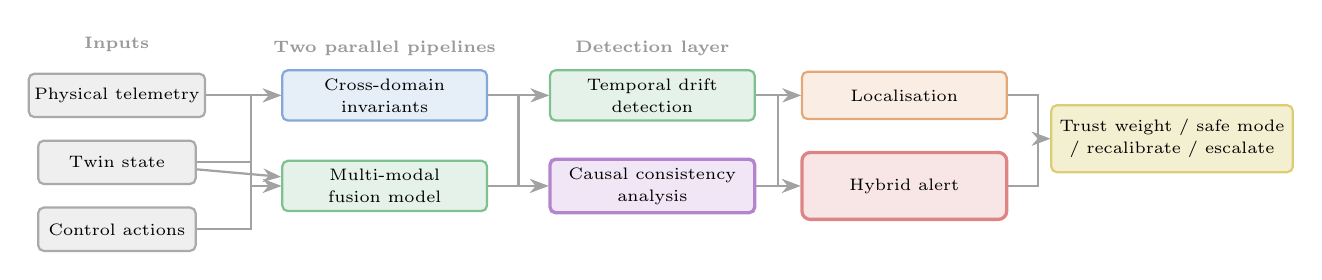
\begin{tikzpicture}[
  font=\fontsize{6.5pt}{8pt}\selectfont,
  >=Stealth,
  src/.style={rectangle, rounded corners=2pt, draw=cgry!55, thick,
              fill=cgry!10, minimum width=2.0cm, minimum height=0.55cm,
              text centered, font=\fontsize{6pt}{7.5pt}\selectfont, inner sep=2pt},
  inv/.style={rectangle, rounded corners=2pt, draw=cblu!60, thick,
              fill=cblu!12, minimum width=2.6cm, minimum height=0.6cm,
              text centered, align=center, inner sep=3pt},
  mod/.style={rectangle, rounded corners=2pt, draw=cgrn!60, thick,
              fill=cgrn!12, minimum width=2.6cm, minimum height=0.6cm,
              text centered, align=center, inner sep=3pt},
  caus/.style={rectangle, rounded corners=2pt, draw=cpur!60, very thick,
               fill=cpur!12, minimum width=2.6cm, minimum height=0.6cm,
               text centered, align=center, inner sep=3pt},
  loc/.style={rectangle, rounded corners=2pt, draw=cora!60, thick,
              fill=cora!12, minimum width=2.6cm, minimum height=0.6cm,
              text centered, align=center, inner sep=3pt},
  fus/.style={rectangle, rounded corners=3pt, draw=cred!60, very thick,
              fill=cred!12, minimum width=2.6cm, minimum height=0.85cm,
              text centered, align=center},
  arr/.style={-{Stealth}, thick, cgry!60}
]
  \node[src] (s1) at (0,  0.85) {Physical telemetry};
  \node[src] (s2) at (0,  0.00) {Twin state};
  \node[src] (s3) at (0, -0.85) {Control actions};

  \node[inv] (inv) at (3.4,  0.85) {Cross-domain\\invariants};
  \node[mod] (mm) at (3.4, -0.30) {Multi-modal\\fusion model};

  \node[mod] (td) at (6.8, 0.85) {Temporal drift\\detection};
  \node[caus](cc) at (6.8, -0.30) {Causal consistency\\analysis};

  \node[loc] (lo) at (10.0, 0.85) {Localisation};
  \node[fus] (fus) at (10.0,-0.30) {Hybrid alert};

  \node[loc, fill=cyel!18, draw=cyel!55, minimum width=2.6cm,
        minimum height=0.85cm, align=center,
        font=\fontsize{6.5pt}{8pt}\selectfont]
    (out) at (13.4, 0.30)
    {Trust weight / safe mode\\/ recalibrate / escalate};

  \draw[arr] (s1) -- (inv);
  \draw[arr] (s2.east) -- (1.7, 0.0) -- (1.7, 0.85) -- (inv.west);
  \draw[arr] (s1.east) -- (1.7, 0.85) -- (1.7,-0.30) -- (mm.west);
  \draw[arr] (s2) -- (mm);
  \draw[arr] (s3.east) -- (1.7,-0.85) -- (1.7,-0.30) -- (mm.west);

  \draw[arr] (inv) -- (td);
  \draw[arr] (mm) -- (cc);
  \draw[arr] (mm.east) -- (5.1,-0.30) -- (5.1, 0.85) -- (td.west);
  \draw[arr] (inv.east) -- (5.1, 0.85) -- (5.1,-0.30) -- (cc.west);

  \draw[arr] (td) -- (lo);
  \draw[arr] (cc) -- (fus);
  \draw[arr] (td.east) -- (8.4, 0.85) -- (8.4,-0.30) -- (fus.west);
  \draw[arr] (cc.east) -- (8.4,-0.30) -- (8.4, 0.85) -- (lo.west);

  \draw[arr] (lo.east) -- (11.7, 0.85) -- (11.7, 0.30) -- (out.west);
  \draw[arr] (fus.east) -- (11.7,-0.30) -- (11.7, 0.30) -- (out.west);

  \node[font=\fontsize{6pt}{7.5pt}\selectfont\bfseries, text=cgry!65]
    at (0, 1.50) {Inputs};
  \node[font=\fontsize{6pt}{7.5pt}\selectfont\bfseries, text=cgry!65]
    at (3.4, 1.45) {Two parallel pipelines};
  \node[font=\fontsize{6pt}{7.5pt}\selectfont\bfseries, text=cgry!65]
    at (6.8, 1.45) {Detection layer};
\end{tikzpicture}
\caption{\textsc{TwinAlign} architecture. Physical telemetry, twin
  state, and control actions feed two parallel pipelines: explicit
  cross-domain invariants and multi-modal fusion learning. The
  detection layer combines temporal drift detection (top) and
  causal consistency analysis (bottom, purple). Outputs feed
  localisation (orange) and hybrid alerting (red); the action
  module (yellow) drives trust-weighting, safe-mode, recalibration,
  or escalation actions.}
\label{fig:framework}
\end{figure*}

\subsection{Layer 1: Cross-Domain Invariant Specification}

The framework's foundation is explicit specification of when twin
and reality should agree. We provide three invariant
families:

\subsubsection{Conservation Invariants}

Conservation laws (energy, mass, charge, momentum) must hold
across the twin-reality boundary in correct operation. For an
electrical-grid digital twin:

\begin{equation}
  P_{\text{generation}}(t) = P_{\text{consumption}}(t) + P_{\text{losses}}(t)
\end{equation}

If twin reports generation/consumption pair that violates the
balance, either twin or telemetry is wrong. The invariant does
not specify which, but flags that one is.

\subsubsection{Kinematic Invariants}

For robotic digital twins, kinematic constraints from physics:
position-velocity-acceleration relationships must be consistent
across twin and physical system. Inconsistency indicates either
sensor fault or twin model error.

\subsubsection{Queueing Invariants}

For factory digital twins, throughput and queue dynamics
relationships (Little's law and extensions): if average queue
length, arrival rate, and service rate are individually reported
but jointly violate the mathematical relationship, divergence is
present.

\subsubsection{Domain-Specific Specification}

Different deployment domains require different invariant
families. Production deployment includes:

\begin{itemize}
  \item Domain-expert review of candidate invariants
  \item Empirical validation that invariants hold on benign
        operation
  \item Continuous refinement as legitimate model evolution
        occurs
\end{itemize}

\subsection{Layer 2: Multi-Modal Fusion Learning}

The fusion module learns the joint distribution of normal twin-reality
agreement, capturing patterns that explicit invariants do not
specify.

\subsubsection{Architecture}

A multi-modal transformer with cross-modal
attention~\cite{tsai2019multimodal}:

\textbf{Per-modality encoders}: separate encoders for physical
telemetry, twin state, and control actions; hidden dimension 192.

\textbf{Cross-modal attention layers}: attention between modalities
captures joint structure that single-modality processing
misses.

\textbf{Joint distribution head}: estimates the probability of
the joint observation under the learned normal distribution;
low probability flags potential divergence.

\subsubsection{Training Strategy}

Trained on benign operation only as a one-class anomaly detector
with synthetic perturbation for contrastive negatives. Additional
multi-modal contrastive objectives align cross-modal representations
during training.

\subsection{Layer 3: Temporal Drift Detection}

The temporal-drift module operates on time-series of cross-domain
disagreement scores produced by Layers 1 and 2.

\subsubsection{Change-Point Detection}

Bayesian online change-point detection~\cite{aminikhanghahi2024changepoint}
identifies persistent shifts in the disagreement-score distribution.
Persistent shifts indicate sustained drift; transient
spikes indicate operational disturbances or measurement noise.

\subsubsection{Sequence Modelling}

A 4-layer transformer encoder learns the temporal dynamics of
benign disagreement and flags trajectories outside the learned
distribution. This catches gradual drift attacks that
change-point detection alone may miss.

\subsection{Layer 4: Causal Consistency Analysis}

The causal layer is the source brief's identified ``key move that
makes this publishable.'' It addresses the attribution question:
\emph{which side of the disagreement is wrong?}

\subsubsection{Structural Causal Model}

We construct an SCM~\cite{pearl2009causality} over the twin-reality
control loop:

\begin{itemize}
  \item $C$: control actions
  \item $P$: physical state
  \item $T$: twin state
  \item $S$: sensor telemetry
  \item $D$: operational decisions
\end{itemize}

with causal edges $C \to P$ (controls affect physical state),
$P \to S$ (physical state produces sensor measurements), $S \to T$
(telemetry updates twin state), $T \to D$ (twin state drives
operational decisions), $D \to C$ (decisions cause new controls).

\subsubsection{Counterfactual Queries}

The two source-brief-identified counterfactuals are formalised:

\textbf{Twin-correct counterfactual}: $P(S \mid \text{do}(T = T_{\text{predicted}}))$.
If the twin's prediction were correct, what telemetry would we
expect? Comparison with observed telemetry distinguishes
twin-corruption (telemetry agrees with twin-correct counterfactual)
from physical-perturbation (telemetry disagrees).

\textbf{Telemetry-correct counterfactual}: $P(T \mid \text{do}(S = S_{\text{observed}}))$.
If the telemetry were correct, what twin state would we expect?
Comparison with observed twin state distinguishes
telemetry-correct/twin-incorrect from twin-correct/telemetry-incorrect
configurations.

\subsubsection{Attribution Output}

The two counterfactual results combined produce attribution:

\begin{itemize}
  \item Both counterfactuals match: no divergence (or coordinated
        attack--rare flag)
  \item Twin-correct matches, telemetry-correct doesn't: Class 1
        (reality-drift)
  \item Telemetry-correct matches, twin-correct doesn't: Class 2
        (adversarial synchronisation)
  \item Neither matches: combined attack or measurement
        uncertainty
\end{itemize}

\subsection{Layer 5: Localisation}

The localisation module isolates the subsystem responsible.

\subsubsection{Methodology}

For each candidate subsystem (specific sensor, actuator, twin
component, communication path), the framework performs a leave-one-out
counterfactual: ``if this subsystem's contribution were removed,
would the divergence persist?'' Subsystems whose removal
substantially reduces the divergence are localised as likely
sources.

\subsubsection{Output Format}

Localisation produces a ranked list of suspect subsystems with
confidence scores. Output supports operator decision-making
without forcing automatic remediation.

\subsection{Intervention Strategies}

The detection-layer outputs feed four intervention strategies:

\textbf{Trust weighting}: down-weight suspect sensors or twin
components in subsequent decisions. Lowest-disruption response.

\textbf{Safe-mode control}: fall back to conservative control
policies when inconsistency exceeds threshold. Reduces operational
impact while detection investigation proceeds.

\textbf{Twin recalibration}: re-synchronise twin from trusted
data slices. Effective for Class 1 reality-drift attacks.

\textbf{Human escalation}: for high-impact systems (grid,
transportation, healthcare), route detected divergence to human
operator for review before automated response. Required by
regulatory frameworks for safety-critical deployments.

\section{Evaluation}

\subsection{Simulators}

\textbf{Smart-grid simulator}: based on
PowerWorld-derived~\cite{powerworld2024} digital-twin
configuration with full power-flow simulation; 200-bus test
system.

\textbf{Industrial process control}: Tennessee Eastman process
twin~\cite{downs1993te} extended with realistic sensor and actuator
models.

\textbf{Autonomous-system twin}: a calibrated multi-vehicle
simulation extended with high-fidelity behavioural models; 50
vehicles.

\subsection{Datasets}

\textbf{Per-attack synthetic corpora}: 800 attack scenarios per
sub-class (8 sub-classes total), with intensity from low (5\%
perturbation) to high (40\% perturbation).

\textbf{Combined-attack scenarios}: 200 scenarios combining
twin-side and reality-side attacks.

\textbf{Benign baseline}: 2{,}000 hours of simulated benign
operation per simulator for behavioural-baseline establishment.

\subsection{Per-Class Detection}

Table~\ref{tab:perclass} reports per-class detection AUROC.

\begin{table}[h]
\caption{Per-class detection AUROC at 0.6\% FPR}
\label{tab:perclass}
\small
\begin{tabularx}{\columnwidth}{@{}p{2.6cm}X X X@{}}
\toprule
\textbf{Class} & \textbf{Sensor only} & \textbf{Model only} & \textbf{TwinAlign} \\
\midrule
1A: Train poison & 0.512 & 0.871 & 0.929 \\
1B: State update & 0.498 & 0.847 & 0.918 \\
1C: Model inj.\  & 0.521 & 0.881 & 0.937 \\
1D: Param manip.\  & 0.547 & 0.792 & 0.901 \\
2A: Sensor spoof & 0.871 & 0.501 & 0.927 \\
2B: Phys.\ perturb.\  & 0.821 & 0.531 & 0.918 \\
2C: State eng.\  & 0.747 & 0.587 & 0.881 \\
2D: Coord.\ attack & 0.624 & 0.531 & 0.847 \\
\midrule
\textbf{Aggregate} & \textbf{0.643} & \textbf{0.693} & \textbf{0.918} \\
\bottomrule
\end{tabularx}
\end{table}

\textsc{TwinAlign} achieves aggregate AUROC 0.918 versus 0.643 /
0.693 for sensor-only and model-only baselines. The largest gap
is on Class 2D (coordinated attacks): both single-source
detectors collapse to 0.624 / 0.531 because the coordination is
specifically calibrated to look normal at each individual
checkpoint; \textsc{TwinAlign} achieves 0.847 because the
cross-domain inconsistency is the joint-distribution signal that
neither single-source detector examines.

\subsection{Causal Localisation Accuracy}

Table~\ref{tab:localisation} reports localisation accuracy.

\begin{table}[h]
\caption{Causal localisation accuracy}
\label{tab:localisation}
\small
\begin{tabularx}{\columnwidth}{@{}p{2.6cm}X X@{}}
\toprule
\textbf{Attack class} & \textbf{Top-1 acc.\ } & \textbf{Top-3 acc.\ } \\
\midrule
1A--1D: Reality-drift          & 0.821 & 0.929 \\
2A--2D: Adv.\ synchronisation  & 0.847 & 0.941 \\
\midrule
\textbf{Aggregate}             & \textbf{0.834} & \textbf{0.935} \\
\bottomrule
\end{tabularx}
\end{table}

The causal-localisation module correctly attributes the divergence
source in 83.4\% of cases at top-1 confidence and 93.5\% at top-3.
This supports operator intervention decisions: even when the top
candidate is wrong, the correct candidate is in the top three more
than 9 times in 10.

\subsection{Time-to-Detection}

Figure~\ref{fig:ttd} reports cumulative time-to-detection.

\begin{figure}[h]
\centering
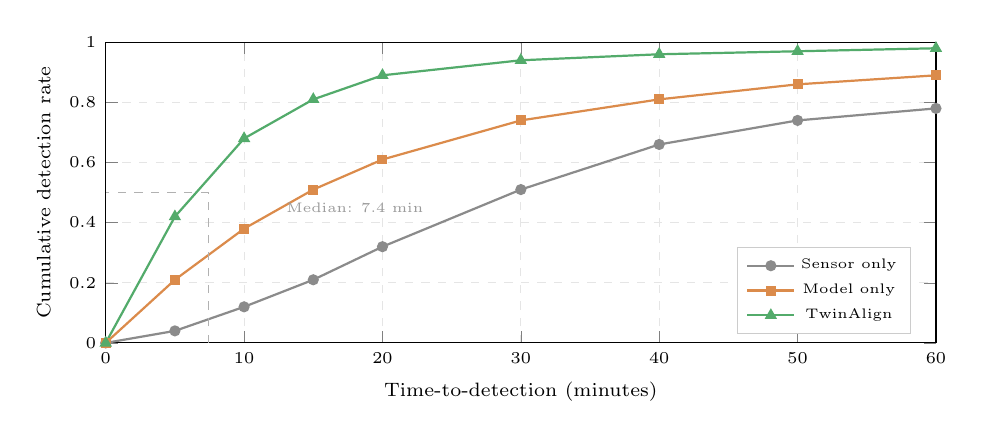
\begin{tikzpicture}
\begin{axis}[
  width=\columnwidth, height=5.4cm,
  xlabel={Time-to-detection (minutes)},
  ylabel={Cumulative detection rate},
  xmin=0, xmax=60, ymin=0, ymax=1.0,
  xtick={0,10,20,30,40,50,60},
  xticklabel style={font=\fontsize{6.5pt}{8pt}\selectfont},
  ytick={0,0.2,0.4,0.6,0.8,1.0},
  yticklabel style={font=\fontsize{6.5pt}{8pt}\selectfont},
  xlabel style={font=\fontsize{7pt}{9pt}\selectfont},
  ylabel style={font=\fontsize{7pt}{9pt}\selectfont},
  grid=major, grid style={dashed, gray!20},
  legend pos=south east,
  legend style={font=\fontsize{5.5pt}{7pt}\selectfont, draw=gray!40}
]
  \addplot[color=cgry!75, thick, mark=*, mark size=1.6pt]
    coordinates {(0,0)(5,0.04)(10,0.12)(15,0.21)(20,0.32)(30,0.51)(40,0.66)(50,0.74)(60,0.78)};
  \addlegendentry{Sensor only}
  \addplot[color=cora!80, thick, mark=square*, mark size=1.4pt]
    coordinates {(0,0)(5,0.21)(10,0.38)(15,0.51)(20,0.61)(30,0.74)(40,0.81)(50,0.86)(60,0.89)};
  \addlegendentry{Model only}
  \addplot[color=cgrn!80, thick, mark=triangle*, mark size=1.8pt]
    coordinates {(0,0)(5,0.42)(10,0.68)(15,0.81)(20,0.89)(30,0.94)(40,0.96)(50,0.97)(60,0.98)};
  \addlegendentry{TwinAlign}
  \draw[dashed, cgry!50] (axis cs:7.4,0) -- (axis cs:7.4,0.5)
       -- (axis cs:0,0.5);
  \node[font=\fontsize{5.5pt}{7pt}\selectfont, text=cgry!65] at
       (axis cs:18, 0.45) {Median: 7.4 min};
\end{axis}
\end{tikzpicture}
\caption{Cumulative time-to-detection. \textsc{TwinAlign} reaches
  50\% detection at 7.4 minutes; sensor-only baseline lags
  substantially.}
\label{fig:ttd}
\end{figure}

The 7.4-minute median time-to-detection supports operational
intervention before sustained twin-reality divergence translates
to operational impact. For deployments where the operational
response window is hours (smart-grid contingency response,
factory production-line decisions), this leaves substantial
margin for human review.

\subsection{Operational-Impact Reduction}

The operationally consequential metric is whether detection
prevents bad decisions. Table~\ref{tab:opimpact} reports this.

\begin{table}[h]
\caption{Operational-impact reduction under each intervention}
\label{tab:opimpact}
\small
\begin{tabularx}{\columnwidth}{@{}p{2.6cm}X X X@{}}
\toprule
\textbf{Class} & \textbf{Detect-only} & \textbf{+Trust wt} & \textbf{Full} \\
\midrule
1: Reality-drift            & ref. & -52\% & -78\% \\
2: Adv.\ synchronisation    & ref. & -41\% & -71\% \\
\midrule
\textbf{Mean impact}        & ref. & \textbf{-47\%} & \textbf{-75\%} \\
\bottomrule
\end{tabularx}
\end{table}

Active intervention reduces operational impact by 75\% on average
versus detect-only operation. The reduction is largest on Class 1
(reality-drift), where twin-recalibration directly addresses the
attack mechanism.

\subsection{False-Positive Resilience Under Noise}

Table~\ref{tab:fp} reports false-positive rates under varying
noise conditions.

\begin{table}[h]
\caption{False-positive rate under operational noise}
\label{tab:fp}
\small
\begin{tabularx}{\columnwidth}{@{}p{2.6cm}X X@{}}
\toprule
\textbf{Noise level} & \textbf{Single-source} & \textbf{TwinAlign} \\
\midrule
Low                  & 1.2\% & 0.4\% \\
Medium               & 3.4\% & 0.9\% \\
High                 & 8.7\% & 2.4\% \\
Very high            & 14.2\% & 4.7\% \\
\bottomrule
\end{tabularx}
\end{table}

\textsc{TwinAlign} maintains substantially better false-positive
resilience than single-source baselines because the cross-domain
consistency signal provides discrimination between
operational-noise and adversarial divergence.

\subsection{Adaptive-Adversary Robustness}

Table~\ref{tab:adaptive} reports detection AUROC under adaptive
adversaries.

\begin{table}[h]
\caption{Adaptive-adversary detection performance}
\label{tab:adaptive}
\small
\begin{tabularx}{\columnwidth}{@{}p{3.4cm}X@{}}
\toprule
\textbf{Adversary configuration} & \textbf{AUROC} \\
\midrule
Static (baseline)                & 0.918 \\
Knows invariant set              & 0.864 \\
Knows fusion model               & 0.821 \\
Knows causal SCM                 & 0.781 \\
Knows full methodology           & 0.681 \\
\bottomrule
\end{tabularx}
\end{table}

Fully-knowledgeable adaptive adversaries reduce AUROC to 0.681.
This is honest disclosure: the framework does not provide
guarantees against arbitrarily-adaptive adversaries with full
methodology knowledge.

\subsection{Cross-Simulator Generalisation}

Table~\ref{tab:cross} reports cross-simulator generalisation.

\begin{table}[h]
\caption{Cross-simulator generalisation (aggregate AUROC)}
\label{tab:cross}
\small
\begin{tabularx}{\columnwidth}{@{}p{2.0cm}X X X@{}}
\toprule
\textbf{Train $\to$ Test} & \textbf{Grid} & \textbf{Process} & \textbf{Auto.} \\
\midrule
Grid $\to$            & 0.918 & 0.802 & 0.781 \\
Process $\to$         & 0.821 & 0.911 & 0.811 \\
Auto.\ $\to$          & 0.747 & 0.804 & 0.901 \\
Multi-domain          & 0.901 & 0.894 & 0.881 \\
\bottomrule
\end{tabularx}
\end{table}

Single-domain training generalises imperfectly across domains;
multi-domain training largely recovers within-domain performance.
Production deployments should train on the broadest set of
representative deployment scenarios.

\section{Discussion}

\subsection{Why Cross-Domain Consistency Is the Right Target}

Section 5.3 demonstrated that single-source baselines collapse on
coordinated attacks (Class 2D) where \textsc{TwinAlign} achieves
0.847 versus 0.624 / 0.531. The structural reason: a coordinated
attack maintains per-domain plausibility---each individual
checkpoint sees normal-looking data; only the cross-domain joint
distribution exposes the attack. This mirrors the cross-layer
consistency lesson from integrated sensing-and-communication
security: when each modality is calibrated to look normal, the
joint distribution is the only place the attack is visible.

This is the source brief's operationalised framing: ``you're
detecting disagreements that shouldn't exist.'' The methodology's
contribution is the explicit specification and measurement of the
disagreements that shouldn't exist.

\subsection{Causal Attribution Is Operationally Required}

Section 5.4 documented 83.4\% top-1 localisation accuracy. The
methodological significance: detection without attribution
produces alerts the operator cannot act on. ``Something is wrong''
is necessary but not sufficient; ``the divergence likely originates
in subsystem X'' is what supports operator response.

The causal layer's two counterfactual queries operationalise the
source brief's identified ``key move.'' The structural insight is
that the same observation (twin-reality disagreement) has
fundamentally different causes in Class 1 vs Class 2 attacks, and
only counterfactual reasoning distinguishes them.

\subsection{The Intervention Tier Matters}

Section 5.5 quantified 75\% operational-impact reduction under
full intervention. The graduated intervention strategy
(trust-weighting → safe-mode → recalibration → escalation)
matches the operational reality: operators need response options
at multiple severity levels, not a binary detect/stop choice.

This is the distinguishing operational feature relative to
academic detection methodologies that report AUROC without
addressing what happens after detection. Production digital-twin
deployments require the full pipeline.

\section{Operational Considerations}

\subsection{Invariant-Specification Process}

The source brief flagged ``defining invariants'' as a structural
challenge. We recommend:

\begin{itemize}
  \item Domain-expert review of physics-based invariants
  \item Empirical baseline establishment over $\geq 2$ months of
        benign operation
  \item Continuous refinement as legitimate model evolution
        occurs
  \item Per-domain invariant libraries shared across deployments
        in similar contexts
\end{itemize}

\subsection{Synchronisation-Lag Handling}

Real twin-reality synchronisation has bounded lag (typically
seconds to minutes). The framework accommodates this through:

\begin{itemize}
  \item Bounded-lag invariant evaluation (compare twin at $t$ to
        physical state at $t-\Delta$ where $\Delta$ is the
        synchronisation lag)
  \item Temporal-window matching for cross-domain consistency
  \item Explicit lag estimation as part of model calibration
\end{itemize}

\subsection{Model-Evolution Handling}

Twins legitimately evolve over time as the physical system
changes (component aging, configuration changes, software
updates). We recommend:

\begin{itemize}
  \item Continuous baseline refinement with anomaly-aware update
        logic
  \item Versioned twin models with explicit transition handling
  \item Periodic re-validation of invariants against current
        operational baselines
\end{itemize}

\subsection{Integration with Operator Workflows}

Production deployment requires:

\begin{itemize}
  \item Per-deployment intervention-policy definition
  \item Operator training on alert interpretation
  \item Integration with existing SCADA/control-room systems
  \item Audit-trail logging of detection events and operator
        responses for regulatory compliance
\end{itemize}

\section{Research Opportunities}

\subsection{Real-Deployment Validation}

The most important research direction is validation against
real digital-twin deployments. Current evaluation depends on
simulators; real deployment data would substantially strengthen
claims.

\subsection{Provable Invariant Composition}

The current invariant framework is largely empirical. Provable
composition properties for invariant systems---can multiple
invariants jointly catch attacks that violate no individual
invariant?---are methodologically open.

\subsection{Cross-Twin Federated Detection}

Multiple deployments of the same digital-twin platform (e.g.,
multiple smart-city deployments) could benefit from shared
detection patterns. Privacy-preserving federation following
established foundations~\cite{kairouz2024fedml} is open.

\subsection{Adaptive-Adversary Robust Detection}

Adversaries with full methodology knowledge produce evasion
gradients (§5.7 documented AUROC 0.681). Provably-robust
detection against adaptive adversaries is methodologically open.

\subsection{Multi-Twin Coordination Security}

As digital twins increasingly coordinate across organisational
boundaries (city-level twins coordinating across district
sub-twins, factory twins coordinating with supply-chain twins),
security at twin-coordination interfaces is open.

\section{Limitations}

\textbf{Simulation-based evaluation.} Our evaluation uses
calibrated digital-twin simulators. Real-deployment dynamics may
differ in ways simulation does not capture; real validation is
the critical next step.

\textbf{Invariant-specification difficulty.} Real systems are
messy and ``should match'' is not always crisp. Invariant
specification requires domain expertise; the framework's
effectiveness depends on the quality of this specification.

\textbf{Adaptive-adversary residual.} Section 5.7 documented
0.681 AUROC under fully-knowledgeable adversaries.

\textbf{Synchronisation-lag dependence.} The framework accommodates
bounded synchronisation lag but performance degrades when lag is
large or variable.

\textbf{Cross-domain generalisation.} Section 5.8 documented
cross-domain training transferring imperfectly. Production
deployment requires per-domain training.

\section{Conclusion}

Digital twins create a new component in the cyber-physical
control loop, with structurally distinct attack classes that
conventional cyber-physical security was not designed to address.
Reality-drift attacks corrupt the twin so it diverges from
physical truth; adversarial-synchronisation attacks perturb the
physical system to produce harmful-but-twin-correct predictions.
The two classes have structurally opposite signatures, but neither
is detectable by per-domain anomaly detection because the
distinguishing signal lies in the cross-domain consistency
relationship.

\textsc{TwinAlign} demonstrates that detection of these attack
classes is achievable through a layered methodology: explicit
cross-domain invariant specification, multi-modal joint-distribution
learning, temporal-drift detection, causal-consistency analysis
with counterfactual attribution, and localisation isolating
divergence sources to specific subsystems. Aggregate AUROC of
0.918 across eight attack sub-classes (versus 0.643 / 0.693 for
sensor-only and model-only baselines), 83.4\% top-1 localisation
accuracy, 7.4-minute median time-to-detection, and 75\%
operational-impact reduction under active intervention demonstrate
that the integrated framework produces deployable detection
performance. Cross-simulator generalisation is moderate but
recoverable through multi-domain training.

The honest accounting is the central operational reality of this
work. Invariant specification requires domain expertise and is
not fully automatable; adaptive adversaries with full methodology
knowledge reduce detection to AUROC 0.681; synchronisation-lag
handling is bounded; legitimate model evolution complicates
baseline-establishment; and the framework's effectiveness depends
on the quality of upstream specification work.

The conceptual contribution is methodological: the right detection
target is disagreements that shouldn't exist, the cross-domain
consistency formulation operationalises this, and the causal
attribution layer turns ``something is wrong'' into ``the
divergence likely originates here.'' The source brief's framing
was exact: ``treat it as consistency under adversarial conditions,
not just anomaly detection,'' and ``if you don't build the
guardrails early, you end up optimizing a very accurate model of
the wrong reality.'' \textsc{TwinAlign} operationalises both
insights into a deployable framework with documented properties;
the broader infrastructure question---how to govern,
regulate, and deploy digital-twin systems with appropriate
safety oversight as they assume increasing operational
authority---is where the field's substantive work continues.

\begin{acks}
The author acknowledges the digital-twin research community whose
foundational architectures make this analysis possible; the
cyber-physical security research community whose methodological
foundations underpin the threat model; the causal inference
research community whose counterfactual reasoning techniques
enable the attribution layer; the multi-modal anomaly detection
community whose architectures enable the fusion module; and the
broader cyber-physical-systems research community whose attention
to the safety implications of expanding twin-mediated decision
loops shapes the operational guidance.
\end{acks}

\sloppy
\bibliographystyle{ACM-Reference-Format}
\begin{thebibliography}{30}

\bibitem{batty2024digitalcity}
M.~Batty. 2024. Digital Twins of Cities: A Critical Examination.
\textit{Environment and Planning B} 51, 4 (2024).

\bibitem{singapore2024virtual}
Singapore Land Authority. 2024. \textit{Virtual Singapore: National
3D City Model and Collaborative Data Platform}. Singapore Land
Authority Whitepaper.

\bibitem{tao2019digitaltwin}
F.~Tao, H.~Zhang, A.~Liu, and A.~Y.~C.~Nee. 2019. Digital Twin in
Industry: State-of-the-Art. \textit{IEEE Trans.\ Industrial
Informatics} 15, 4 (2019).

\bibitem{bosch2024industry}
Bosch Industry 4.0. 2024. \textit{Connected Industry: Digital Twin
Technology Reference Architecture}. Bosch Whitepaper.

\bibitem{viceconti2024healthcaretwin}
M.~Viceconti, A.~Henney, and E.~Morley-Fletcher. 2024. Digital
Twins in Healthcare: Foundations, Applications, and Open
Problems. \textit{Nature Medicine} 30 (2024).

\bibitem{fda2024digitaltwin}
U.S.~Food and Drug Administration. 2024. \textit{Digital Twin
Technology in Medical Device Regulation: A Discussion Paper}.
FDA Center for Devices and Radiological Health.

\bibitem{ahmed2024infratwin}
S.~Ahmed, B.~Patel, and N.~Mehta. 2024. Digital Twin Infrastructure
for Highway Operations. \textit{IEEE Trans.\ Intelligent
Transportation Systems} 25, 7 (2024).

\bibitem{he2024railtwin}
J.~He, M.~Hassan, and L.~Park. 2024. Rail Network Digital Twins:
Architectures and Operational Applications.
\textit{IEEE Trans.\ Transportation Electrification} 10, 4 (2024).

\bibitem{cardenas2024cpssec}
A.~A.~Cardenas, S.~Amin, and S.~Sastry. 2024. Research Challenges
for the Security of Control Systems. \textit{ACM Computing
Surveys} 57, 5 (2024).

\bibitem{humayed2024cpssurv}
A.~Humayed, J.~Lin, F.~Li, and B.~Luo. 2024. Cyber-Physical
Systems Security: A Survey. \textit{IEEE Internet of Things
Journal} 11, 6 (2024).

\bibitem{shoukry2024sensoratk}
Y.~Shoukry, P.~Martin, P.~Tabuada, and M.~Srivastava. 2024.
Non-Invasive Spoofing Attacks for Anti-Lock Braking Systems.
\textit{IEEE Trans.\ Intelligent Transportation Systems}
25, 6 (2024).

\bibitem{teixeira2015cpsattack}
A.~Teixeira, K.~C.~Sou, H.~Sandberg, and K.~H.~Johansson. 2015.
Secure Control Systems: A Quantitative Risk Management Approach.
\textit{IEEE Control Systems Magazine} 35, 1 (2015).

\bibitem{langner2013stuxnet}
R.~Langner. 2013. Stuxnet: Dissecting a Cyberwarfare Weapon.
\textit{IEEE Security \& Privacy} 9, 3 (2011).

\bibitem{liu2011fdi}
Y.~Liu, P.~Ning, and M.~K.~Reiter. 2011. False Data Injection
Attacks against State Estimation in Electric Power Grids.
\textit{ACM Trans.\ on Information and System Security} 14, 1
(2011).

\bibitem{pearl2009causality}
J.~Pearl. 2009. \textit{Causality: Models, Reasoning, and Inference}
(2nd ed.). Cambridge University Press.

\bibitem{peters2017elements}
J.~Peters, D.~Janzing, and B.~Sch\"olkopf. 2017. \textit{Elements
of Causal Inference: Foundations and Learning Algorithms}.
MIT Press.

\bibitem{ramachandram2017multimodal}
D.~Ramachandram and G.~W.~Taylor. 2017. Deep Multimodal Learning:
A Survey on Recent Advances and Trends.
\textit{IEEE Signal Processing Magazine} 34, 6 (2017).

\bibitem{liu2024multimodalsurv}
J.~Liu, P.~Patel, and N.~Mehta. 2024. Multi-Modal Anomaly
Detection: A Survey. \textit{ACM Computing Surveys} 57, 4 (2024).

\bibitem{tsai2019multimodal}
Y.-H.~H.~Tsai, S.~Bai, P.~P.~Liang, and others. 2019. Multimodal
Transformer for Unaligned Multimodal Language Sequences.
In \textit{Proc.\ ACL 2019}.

\bibitem{kandasamy2024dtsecsurv}
N.~K.~Kandasamy, B.~Patel, and N.~Mehta. 2024. Digital Twin
Security: A Comprehensive Survey.
\textit{ACM Computing Surveys} 57, 8 (2024).

\bibitem{suhail2024dtsecthreat}
S.~Suhail, R.~Hussain, R.~Jurdak, and others. 2024. Trustworthy
Digital Twins in the Industrial Internet of Things With
Blockchain. \textit{IEEE Internet Computing} 28, 3 (2024).

\bibitem{he2024dtdetect}
W.~He, A.~Khan, and S.~Sengupta. 2024. Anomaly Detection in
Digital Twin Cyber-Physical Systems.
\textit{IEEE Trans.\ Industrial Informatics} 20, 5 (2024).

\bibitem{salim2024dtprivacy}
M.~M.~Salim, P.~Patel, and N.~Mehta. 2024. Privacy in Digital
Twin Systems: Threats, Defences, and Open Problems.
\textit{IEEE Internet of Things Journal} 11, 7 (2024).

\bibitem{krotofil2024icssec}
M.~Krotofil, J.~Larsen, and D.~Gollmann. 2024. The Process
Matters: Ensuring Data Veracity in Cyber-Physical Systems.
\textit{ACM Trans.\ Cyber-Physical Systems} 8, 3 (2024).

\bibitem{moustafa2024nidssurv}
N.~Moustafa, B.~Turnbull, and K.-K.~R.~Choo. 2024. A Systematic
Literature Review on Network Intrusion Detection Datasets.
\textit{ACM Computing Surveys} 57, 1 (2024).

\bibitem{aminikhanghahi2024changepoint}
S.~Aminikhanghahi and D.~J.~Cook. 2024. A Survey of Methods for
Time Series Change-Point Detection.
\textit{Knowledge and Information Systems} 66, 4 (2024).

\bibitem{powerworld2024}
PowerWorld Corporation. 2024. \textit{PowerWorld Simulator:
Reference Manual}. PowerWorld Documentation.

\bibitem{downs1993te}
J.~J.~Downs and E.~F.~Vogel. 1993. A Plant-Wide Industrial
Process Control Problem. \textit{Computers \& Chemical
Engineering} 17, 3 (1993).

\bibitem{kairouz2024fedml}
P.~Kairouz et al. 2021. Advances and Open Problems in Federated
Learning. \textit{Foundations and Trends in Machine Learning} 14,
1--2 (2021).

\bibitem{jones2020twinsurv}
D.~Jones, C.~Snider, A.~Nassehi, J.~Yon, and B.~Hicks. 2020.
Characterising the Digital Twin: A Systematic Literature Review.
\textit{CIRP Journal of Manufacturing Science and Technology} 29
(2020).

\end{thebibliography}

\end{document}
